\documentclass[xcolor=dvipsnames]{beamer} 
\usetheme{Madrid}
\usepackage{booktabs}
\usepackage[T1]{fontenc}
\usepackage{pifont}
\usepackage{setspace}% http://ctan.org/pkg/setspace
\let\oldframetitle\frametitle% Store old \frametitle in \oldframetitle
\renewcommand{\frametitle}[1]{% Redefine \frametitle
	\oldframetitle{#1}\setstretch{1.25}}
\usepackage{natbib}
\bibpunct{(}{)}{;}{a}{}{,}
\usefonttheme{serif}
\usefonttheme{professionalfonts}
\usepackage{amsmath, tgpagella, eulerpx, eucal, hyperref, bookmark}
\usepackage{tikz}
\usetikzlibrary{through,calc,angles,quotes, arrows.meta,patterns,intersections}
\useoutertheme{miniframes} 
\useinnertheme{circles}
\definecolor{darkred}{rgb}{0.55, 0.0, 0.0}
\usecolortheme[named=darkred]{structure} % you can change colortheme here

\title{Economic Development}
\date{\today}
\author[Sanghoon Park]{Sanghoon Park \newline \newline  \footnotesize{Ph.D. Student}}
\institute[UofSC]{Department of Political Science}
\titlegraphic{
\includegraphics[width=4cm]{UofSC_Primary_RGB_G}}
\usepackage{Sweave}
\begin{document}
\Sconcordance{concordance:R4_Economic_Development.tex:R4_Economic_Development.Rnw:%
1 26 1 1 0 367 1}

	
	\begin{frame}
		\titlepage
	\end{frame}
	\begin{frame}
		\tableofcontents
	\end{frame}

% Overviews
	
	\section{Before We Start}
	\subsection{Causality}
	\begin{frame}[fragile]{$X$ causes $Y$}
	\begin{itemize}
	  \item $X$ covaries with $Y$. \pause
	  \item $X$ causes $Y$. \pause
	  \item Covariation does not prove causality.
	  \item Some examples of covariation without causality.
	  \begin{itemize}
	    \item The crime rate in the South African Republic and the military spending in the U.S.
	    \item The birth rates in South Korea and the number of polar bears.
	   \end{itemize}
	\end{itemize}
	\end{frame}

	\begin{frame}[fragile]{Five Causal Hurdles}
	\begin{enumerate}
	  \item We need a credible causal mechanism.
	  \begin{itemize}
	    \item Answer the ``how" and ``why" questions.
	    \item Only if ``yes," we can move on.
	  \end{itemize}
	  \item $X$ (cause) must come before $Y$ (outcome) in time (Temporal order).
	  \item More of $X$ is associated with more or less of $Y$ (Covariation).
	\end{enumerate}
	\end{frame}
	
	\begin{frame}[fragile]{Five Causal Hurdles}
	\begin{enumerate}
	\setcounter{enumi}{3}
	  \item Endogeneity \pause
	  \begin{itemize}
	    \item $Y$ must cause $X$.
	    \item ``Do the strong survive or are survivors strong?"
	    \item $X \rightarrow Y$ or $Y \rightarrow X$?
	    \item ``Endogenous" means that $A$ causes changes in $B$, but that $B$ also causes changes in $A$.
	  \end{itemize} 
	\end{enumerate}
  \end{frame}

	\begin{frame}[fragile]{Five Causal Hurdles}
	
		\begin{columns}[T]
			\begin{column}{0.6\textwidth}
				\begin{figure}
	        \centering
	        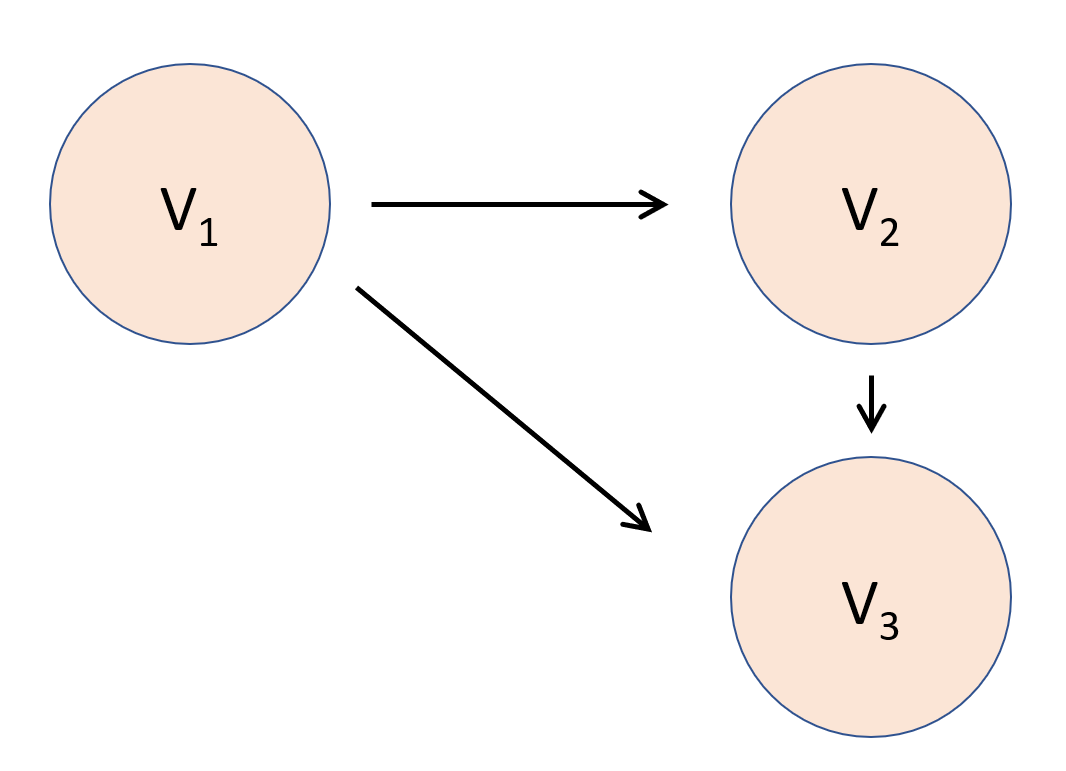
\includegraphics[width=0.8\linewidth]{endogeneity.png}
        	\caption{Endogeneous vs. Exogenous}
	        \label{fig2}
	      \end{figure}
			\end{column}
			
			\begin{column}{0.36\textwidth}
			\end{column}
		\end{columns}
	\end{frame}


	\begin{frame}[fragile]{Five Causal Hurdles}
		\begin{columns}[T]
			\begin{column}{0.6\textwidth}
				\begin{figure}
	        \centering
	        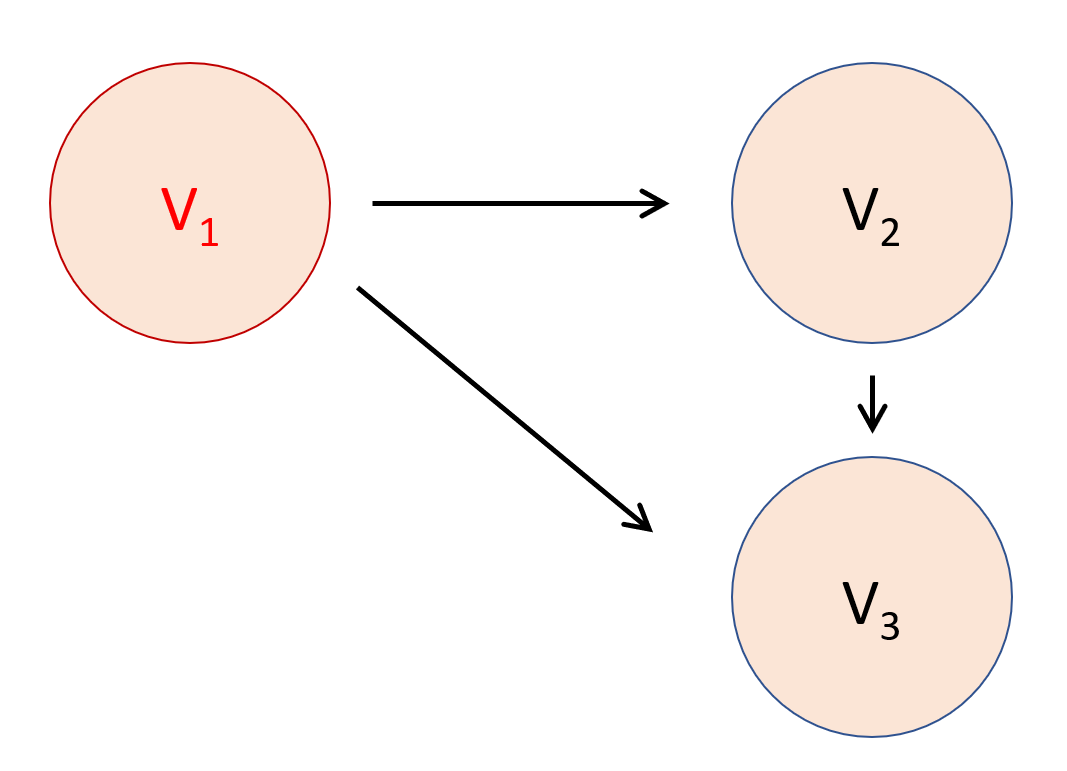
\includegraphics[width=0.8\linewidth]{endogeneity2.png}
        	\caption{Endogeneous vs. Exogenous}
	        \label{fig3}
	      \end{figure}
			\end{column}
			
	\begin{column}{0.36\textwidth}
			\begin{itemize}
			  \item[]
			  \item[]
			  \item $V_1$: Exogenous (given)
			 \end{itemize}
			\end{column}
		\end{columns}
	\end{frame}
	
	\begin{frame}[fragile]{Five Causal Hurdles}
		\begin{columns}[T]
			\begin{column}{0.6\textwidth}
				\begin{figure}
	        \centering
	        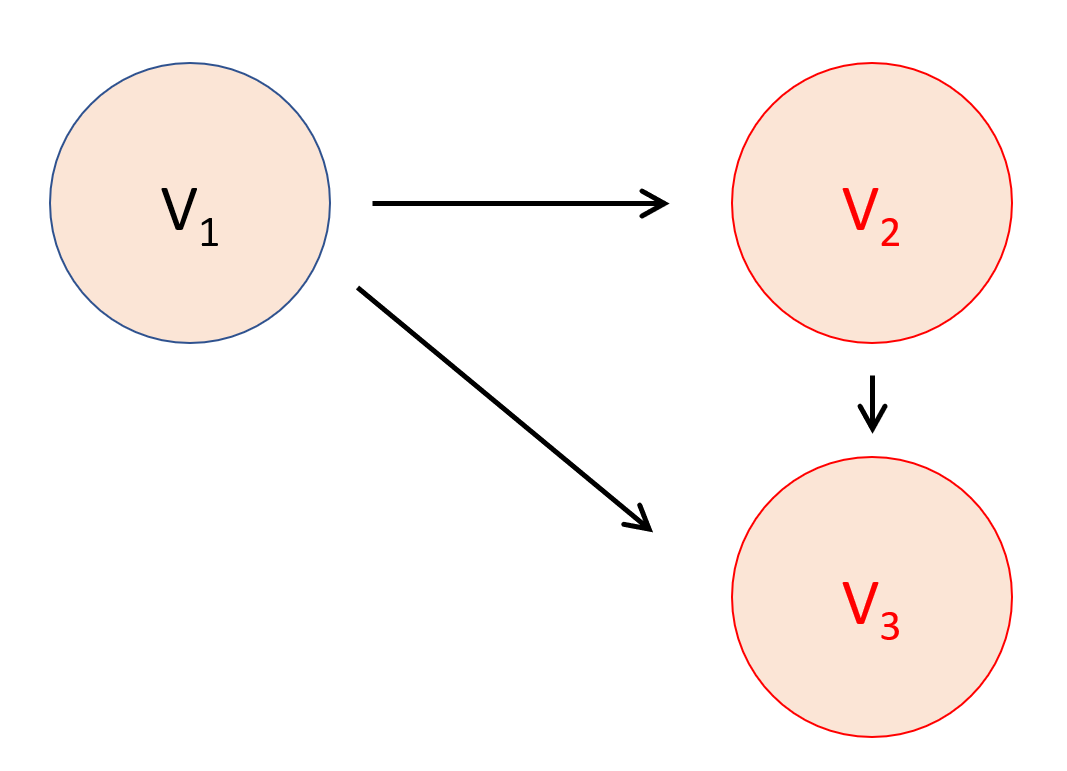
\includegraphics[width=0.8\linewidth]{endogeneity3.png}
        	\caption{Endogeneous vs. Exogenous}
	        \label{fig4}
	      \end{figure}
			\end{column}
			
			\begin{column}{0.36\textwidth}
			\begin{itemize}
			  \item[]
			  \item[]
			  \item $V_1$: Exogenous (given)
			  \item $V_2$, $V_3$: Endogenous (affected)
			\end{itemize}
			\end{column}
		\end{columns}
	\end{frame}


	\begin{frame}[fragile]{Five Causal Hurdles}
  \begin{enumerate}
  \setcounter{enumi}{4}
	  \item Spuriousness
	  \begin{itemize}
	    \item Omitted variable bias
	    \item Some unindentified factor is responsible for the relationship between $X$ and $Y$.
	    \item Thus, spuriousness means that you might think that one thing ($A$) is causing another ($B$), but it's because you ignore what is actually causing the changes.
	  \end{itemize}
	\end{enumerate}
	\end{frame}
	
	\begin{frame}[fragile]{Five Causal Hurdles}
	\begin{figure}
  \centering
  \begin{tikzpicture}
	
	\draw[-{Triangle[scale=1]}, thick] (0,0)--(6,0);
	\node[left] at (0,0.1){X};
	\draw[-{Triangle[scale=1]}, thick] (3.1,4) --(0,0.2);
	\node[above] at (3.1,4){Z};
	\draw[-{Triangle[scale=1]}, thick] (3.2,4)--(6.2,0.1);
	\node[right] at (6.3,0.1){Y};
	
  \end{tikzpicture}
  \caption{Spurious relationship}
  \label{fig1}
  \end{figure}
	\end{frame}
	
	\begin{frame}[fragile]{Five Causal Hurdles}
	\begin{itemize}
	  \item \citet{wucherpfennig:Deutsch:2009} and \citet{boix:stokes:2003} also address the causal issue.
	  \begin{itemize}
	    \item Economic Development $\rightarrow$ Democracy? \pause
	    \item Economic Development $\rightarrow$ Democracy $\rightarrow$ Economic Development?
  	  \item Democracy $\rightarrow$ Economic Development?
  	 \end{itemize}
  	\item This topic is still on the debate since it is challenging to demonstrate the causality of the relationship.
	\end{itemize}
	\end{frame}
	
	% Wucherpfenning, Julian, and Franziska Deutsch. 2009. "Modernization and Democracy: Theories and Evidence Revisited." Living Reviews in Democracy 1: 1-9.
	\section{Wucherpfenning and Deutsch. 2009.}
	\subsection{Modernization and Democracy: Theories and Evidence Revisited}
	
	\begin{frame}[fragile]{General question}
		\begin{columns}[T]
			\begin{column}{0.4\textwidth}
				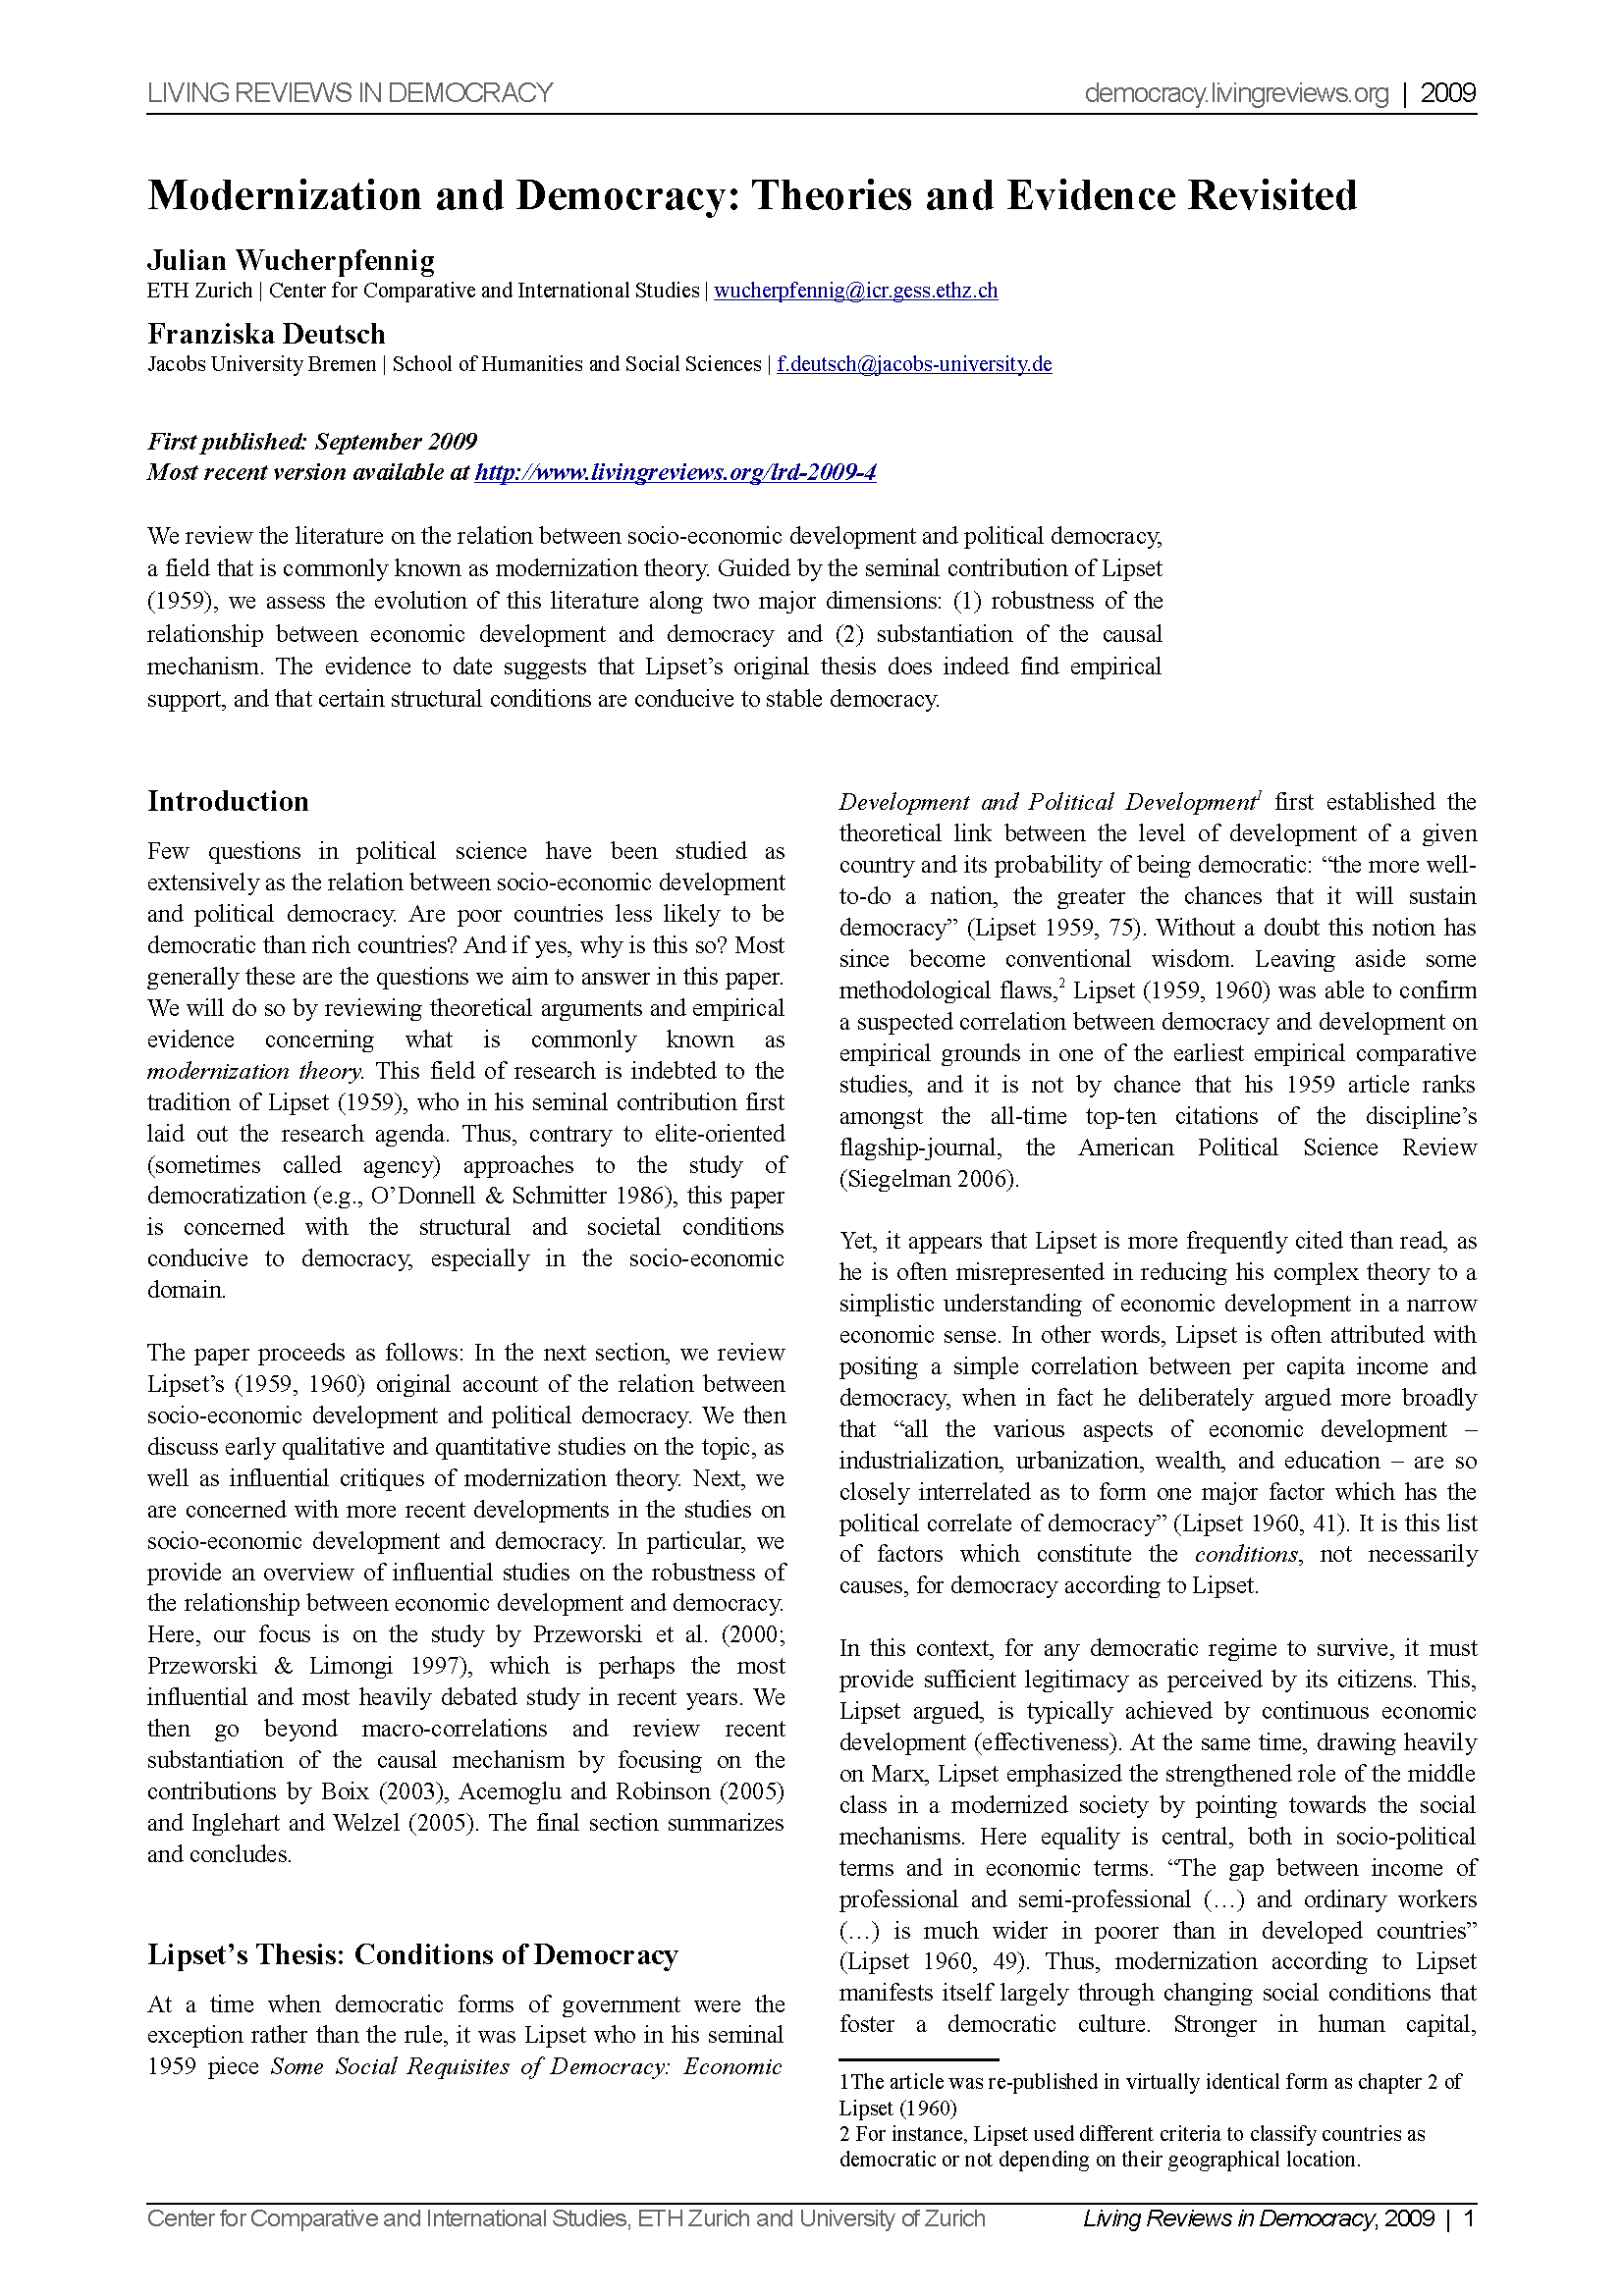
\includegraphics[width=0.8\linewidth]{WucherpfenningDeutch2009.png}
			\end{column}
			
			\begin{column}{0.56\textwidth}
				\begin{center}
					\textit{\textcolor{blue}{Question:}}\\ \pause
					\bigskip		
					What is the relationship between socio-economic development and political democracy?\\ \pause
					\bigskip		
					Are poor countries less likely to be democratic than rich countries?
				\end{center}
			\end{column}
		\end{columns}
	\end{frame}
	
	\begin{frame}[fragile]{Theories}
	\begin{itemize}
		\item Modernization theory \citep{lipset:1959}
			\begin{itemize}
				\item Development $\rightarrow$ the likelihood of democratization $\uparrow$ \pause
				\item Also, development $\rightarrow$ stable democracy $\uparrow$ \pause
				\item Here, development means:
				\begin{enumerate}
				  \item Industrialization
				  \item Urbanization
				  \item Wealth
				  \item Education
				\end{enumerate}
			\end{itemize}
		\end{itemize}
	\end{frame}
	
	\begin{frame}[fragile]{Theories}
	\begin{figure}
	\centering
	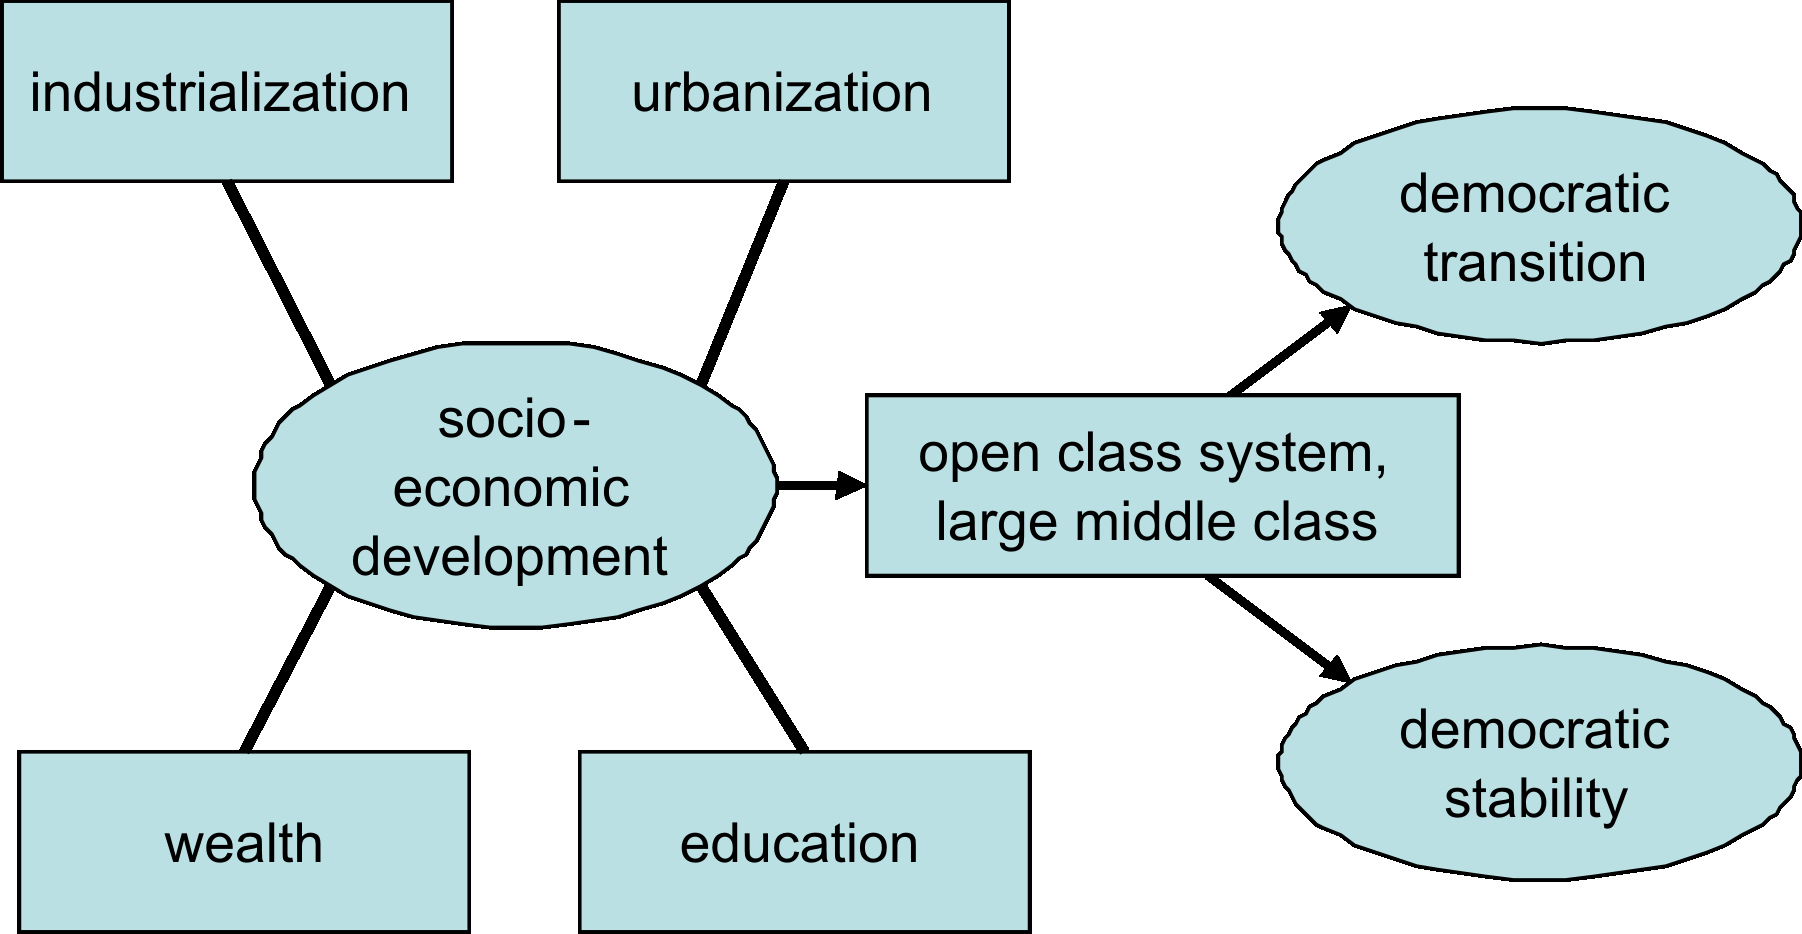
\includegraphics{modernization theory.png}
	\caption{Modernization theory of Lipset (1959)}
	\end{figure}
	\end{frame}
	
\begin{frame}[fragile]{Theories}
	\begin{itemize}
		\item \citet{przeworskietal:2000}
    \begin{itemize}
      \item Exogenous holds, but endogenous fails.
        \begin{itemize}
          \item Economic development does not casue democratization.
          \item Development merely helps sustain democracy once it is established  \citep[3]{wucherpfennig:Deutsch:2009}.
        \end{itemize}
      \item Using 1950-1990, 135 countries data.
    \end{itemize}
	\end{itemize}
\end{frame}
	
% Boix, Carles, and Susan C. Stokes. 2003. "Endogenous Democratization." World Politics 55(4): 517-549.
	
	\section{Boix and Stokes. 2003.}
	\subsection{Endogenous Democratization}
	
	\begin{frame}[fragile]{General question}
		\begin{columns}[T]
			\begin{column}{0.4\textwidth}
				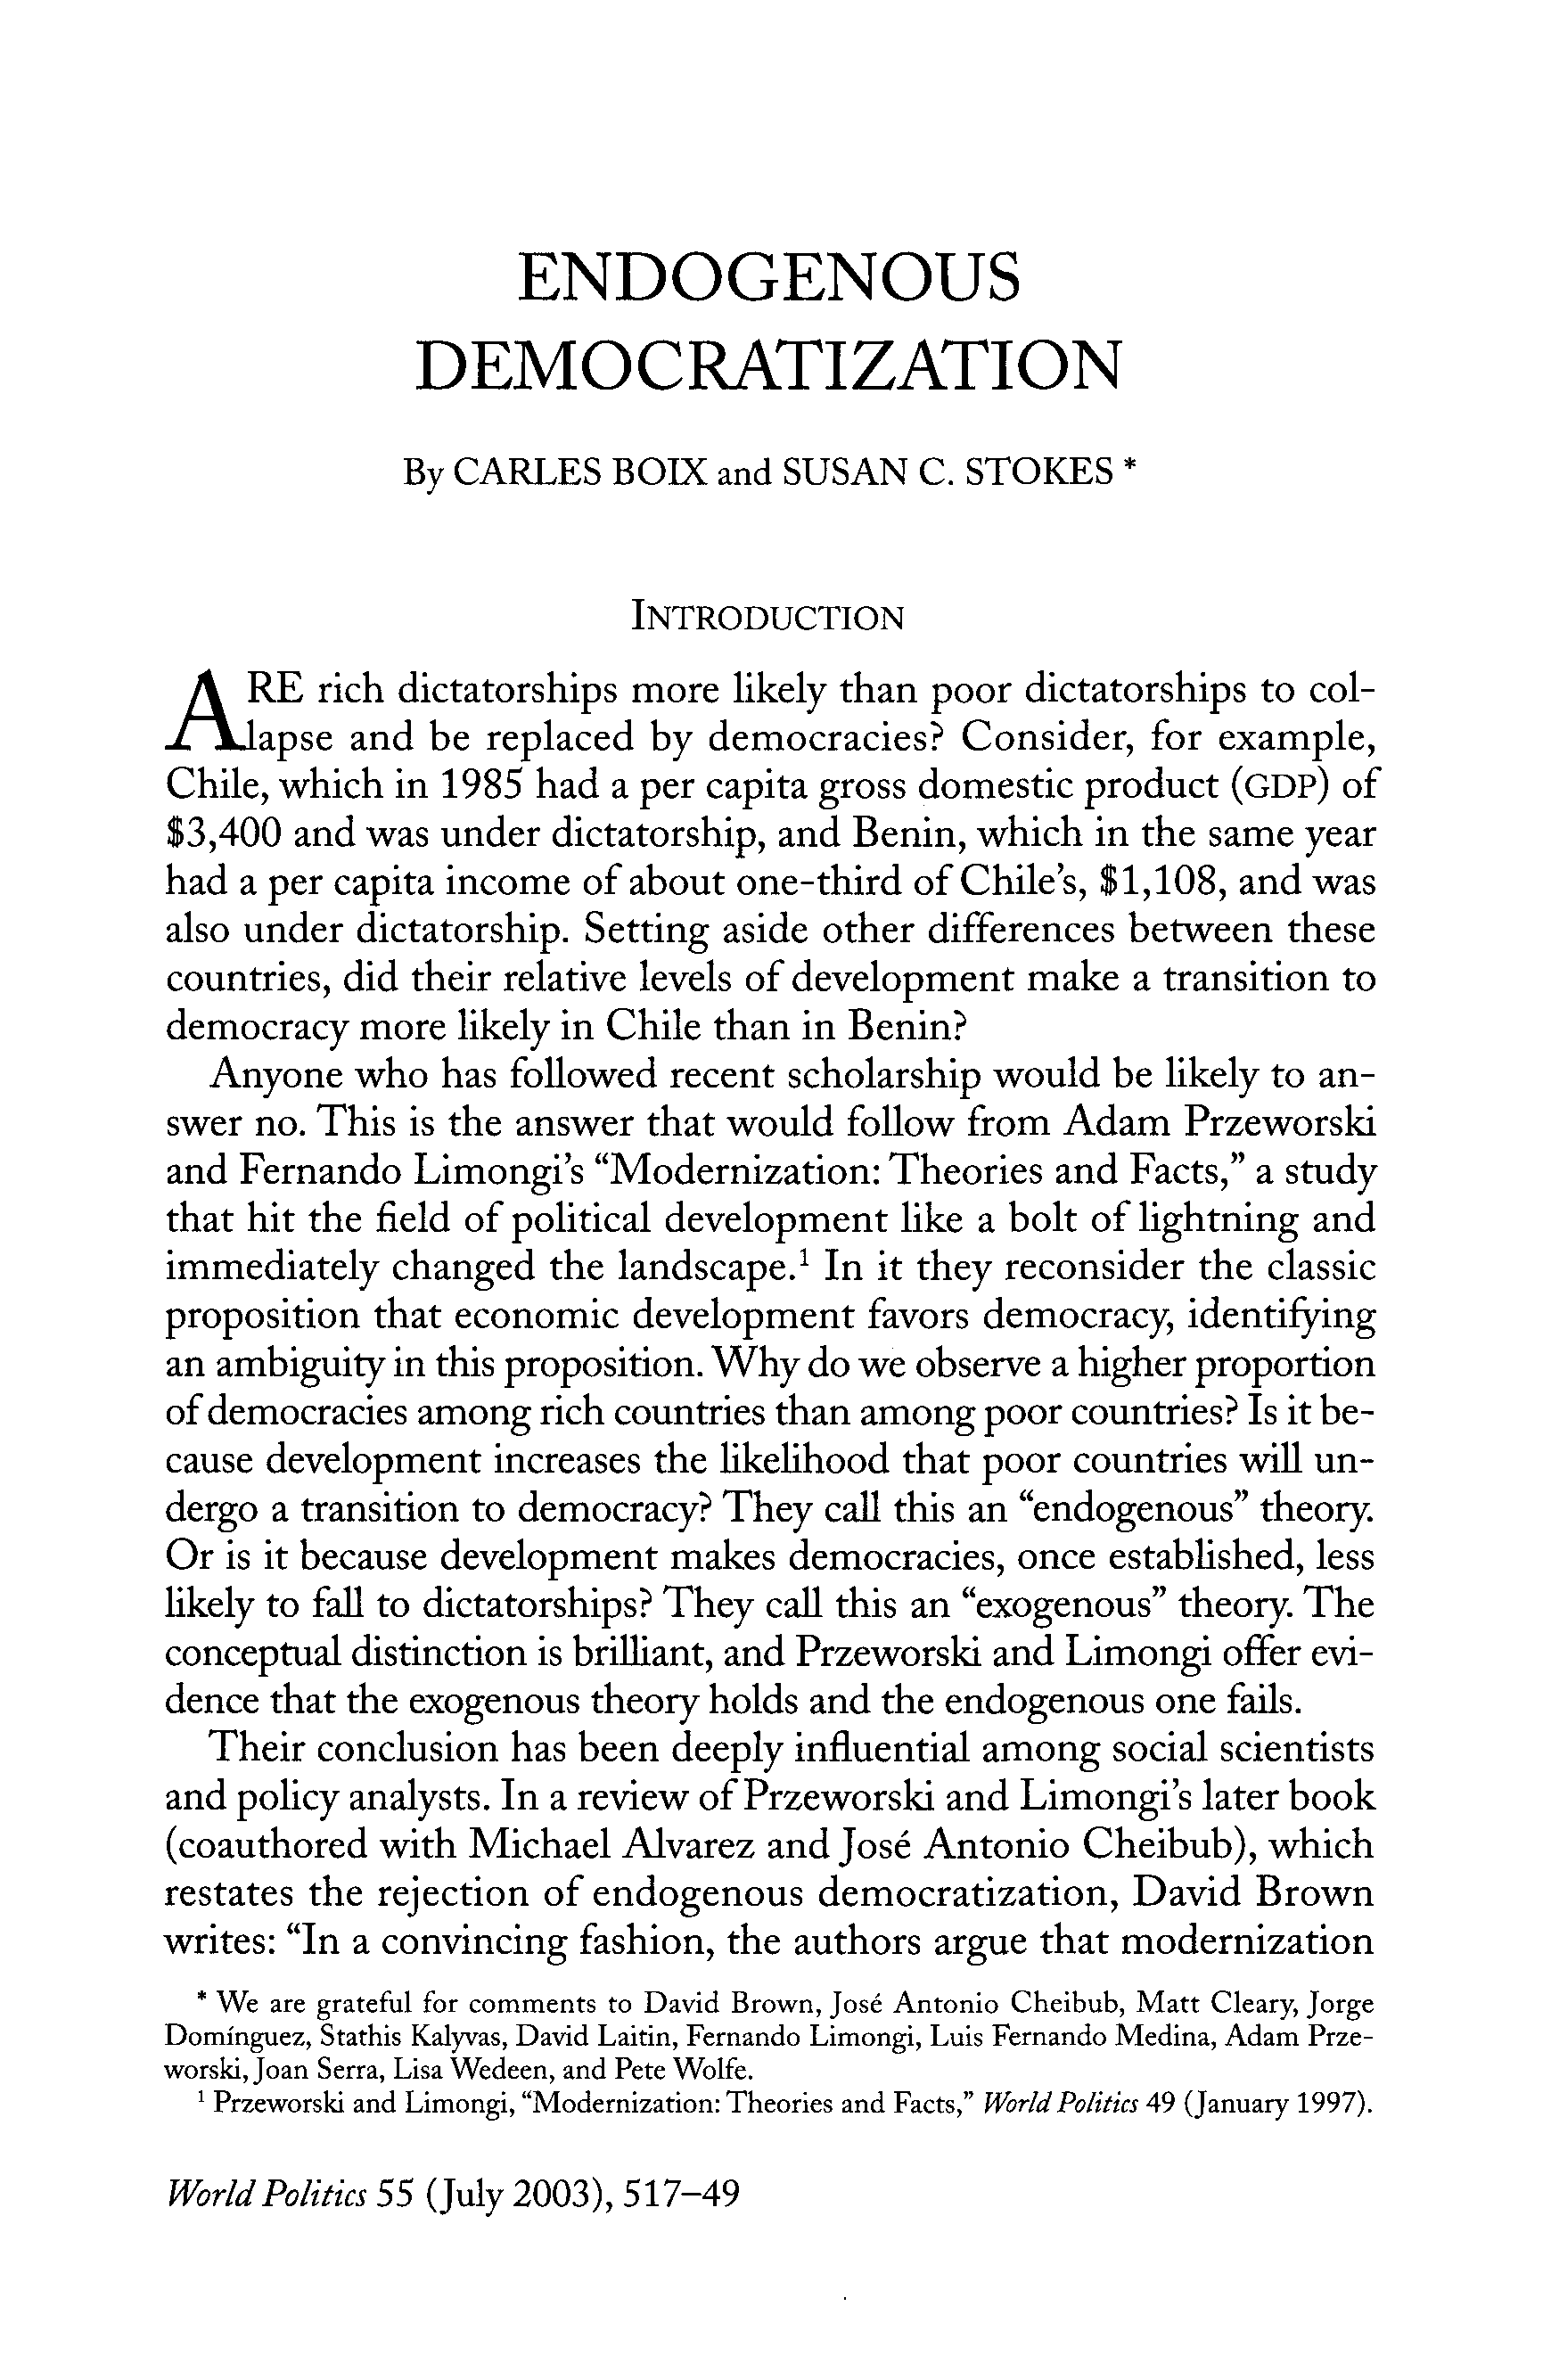
\includegraphics[width=0.8\linewidth]{BoixStokes2003.png}
			\end{column}
			
			\begin{column}{0.56\textwidth}
				\begin{center}
					\textit{\textcolor{blue}{Question:}}\\ \pause
					\bigskip		
					Are rich dictatorships more likely than poor dictatorships to collapse and be replaced by democracies? 
				\end{center}
			\end{column}
		\end{columns}
	\end{frame}
	
	\begin{frame}[fragile]{Theories}
	\begin{figure}
	\centering
	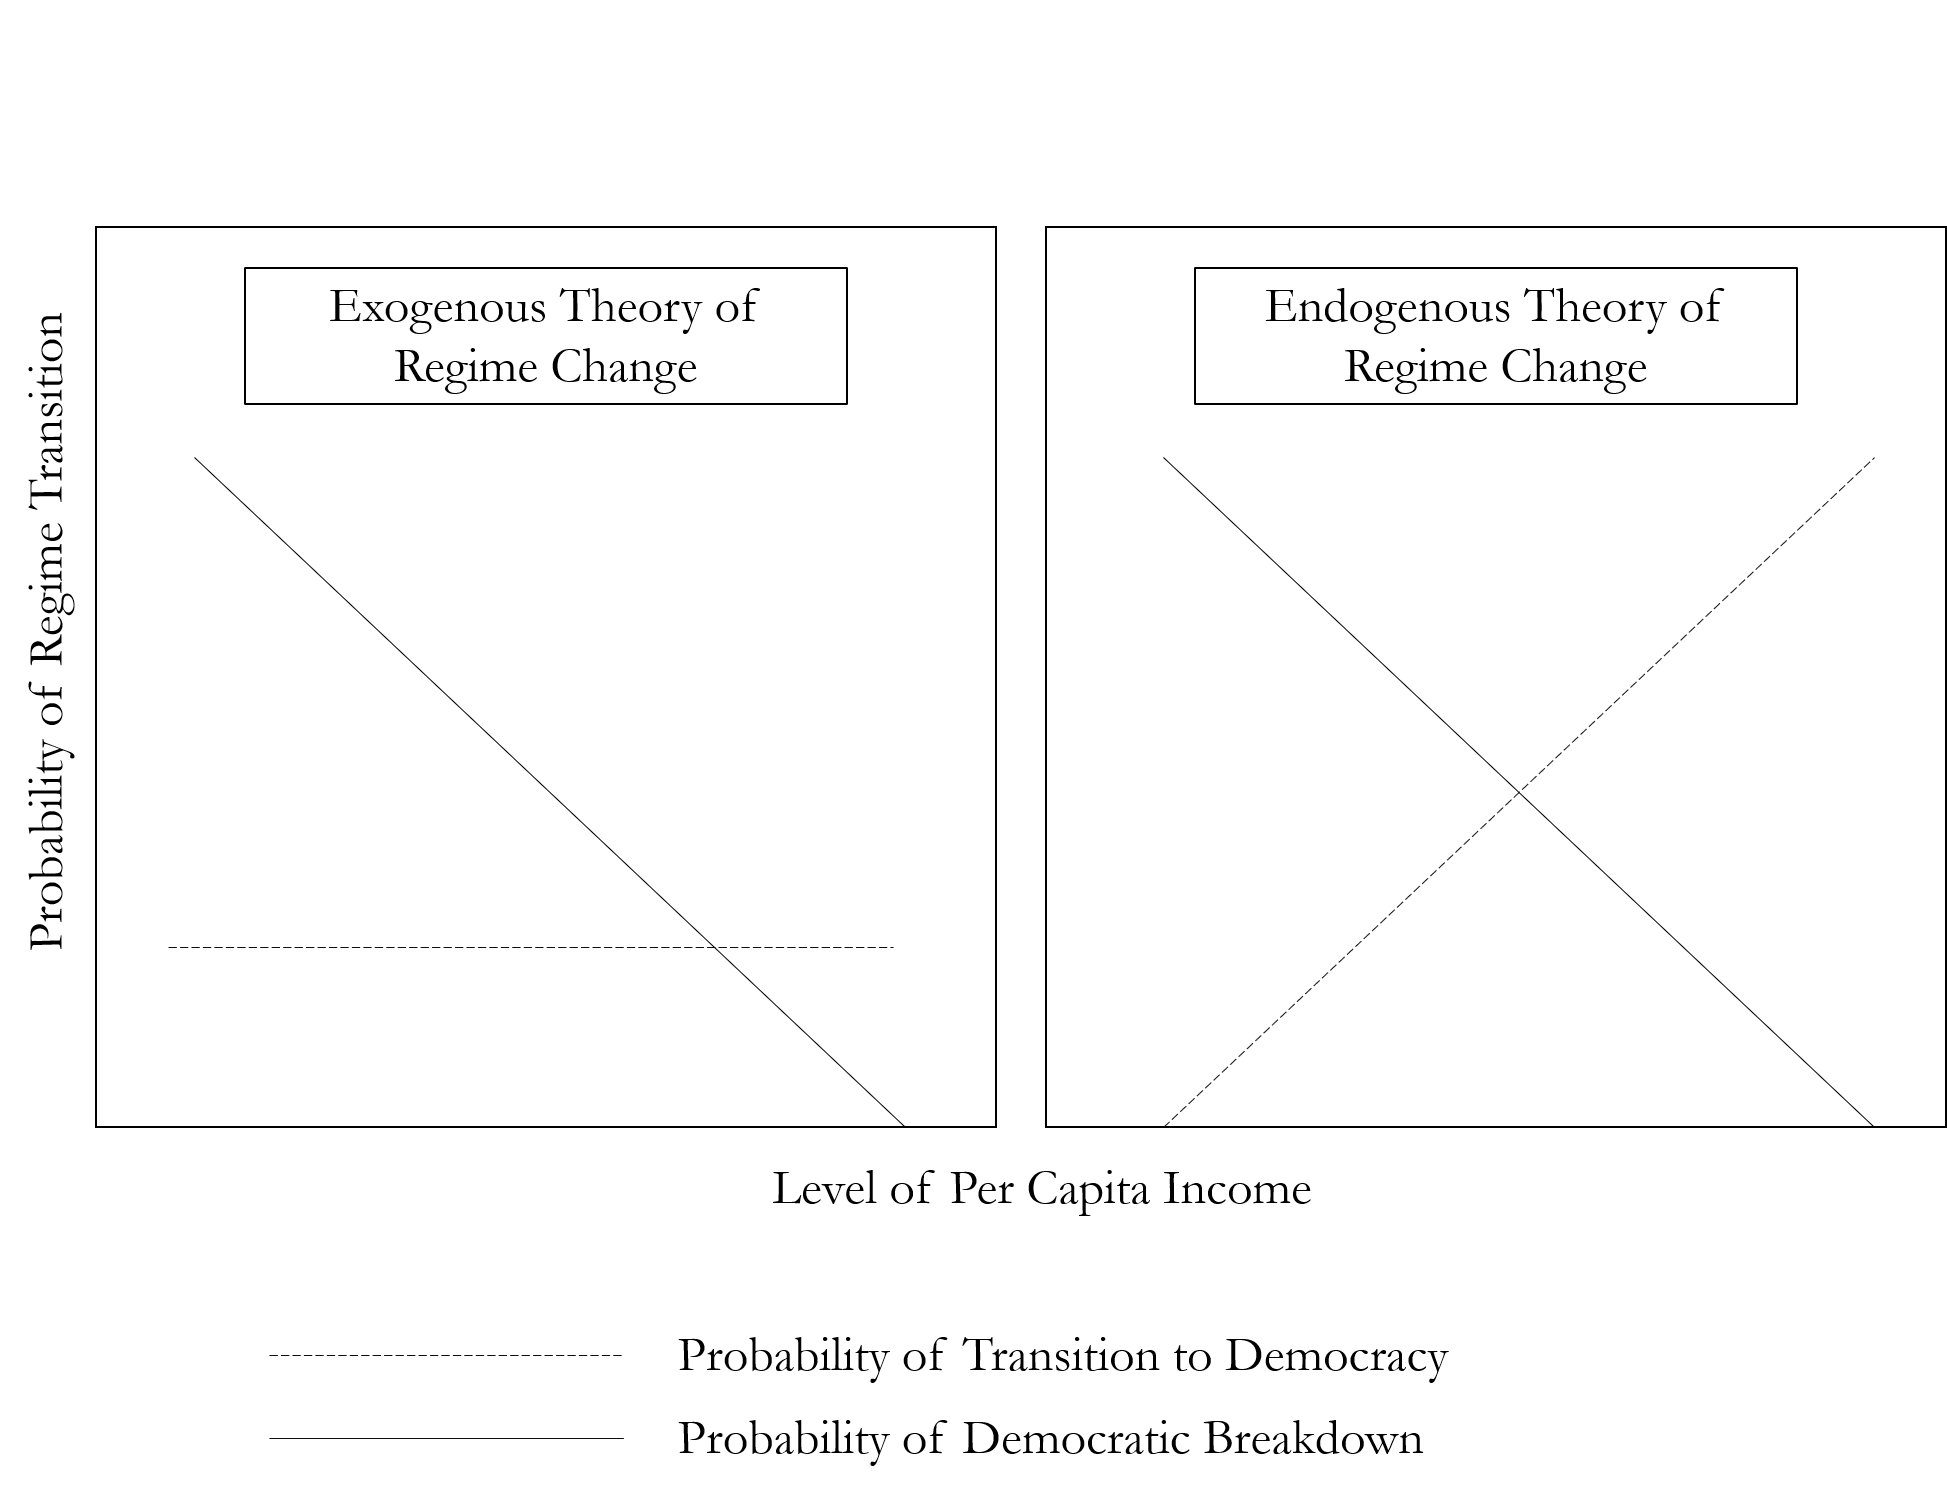
\includegraphics[width=0.6\linewidth]{theoretical.png}
	\caption{The Exogenous and Endogenous Theory of Regime Change}
	\end{figure}
	\end{frame}
	
	\begin{frame}[fragile]{Theories}
	\begin{itemize}
	  \item If the exogenous theory holds, 
	   \begin{itemize}
	    \item Development $\nrightarrow$ Democracy
	    \item But development $\rightarrow$ Stable/developed democracy
	   \end{itemize}
	  \item We need a theory in which development induces actors in democracies to sustain that system but does not induce actors in a dictatorship to change to democracy.
	   \item \citet{boix:stokes:2003} revisit modernization theory--endogenous theory.
	\end{itemize}
	\end{frame}
	
	
	\begin{frame}[fragile]{Empirical Analyses}
	\begin{itemize}
	  \item Theoretical reviews and empirical tests
	  \begin{itemize}
	  \item Are the results of \citet{przeworskietal:2000} generalizable? \pause $\rightarrow$ Expanding the sample.\pause
	  \item When \citet{boix:stokes:2003} expand the sample, do the results cover \citet{przeworskietal:2000}'s? \pause $\rightarrow$ Re-estimate and compare.\pause
	  \item Do \citet{przeworskietal:2000}'s model capture a set of relevant variables? \pause $\rightarrow$ Omitted variable bias \pause
	  \item Do they miss something to infer the causality? \pause $\rightarrow$ Possible causal mechanism: \textit{Inequality}
	  \end{itemize}
	 \end{itemize}
\end{frame}

\begin{frame}[fragile]{Empirical Analyses}
	\begin{itemize}
	\item How does inequality work in the relationship between development and democratization?\\(Development $\rightarrow$ Democratization)
	  \begin{itemize}
	    \item Actors in democracy (gets more under democracy)
	    \item Actors in poor authoritarianism
	    \begin{itemize}
	      \item Equally poor on average
	      \item Democratization $\rightarrow$ Expected benefits are small.
	     \end{itemize}
	   \item Actors in wealthy authoritarianism
	   \begin{itemize}
	      \item High inequality (elites monopolize)
	      \item Democratization $\rightarrow$ Redistributes more.
	      \item Likely transition to democracy.
	   \end{itemize}
	  \end{itemize}
	\end{itemize}
\end{frame}

	
\begin{frame}[fragile]{Empirical Analyses}
	\begin{itemize}	
	 \item Sample \& Methods
	 \begin{itemize}
	  \item Countries from 1850 to 1990.
	  \item Unit of analysis: country-year
	  \item Method: Quantitative analysis
	 \end{itemize} 
	 \item Findings
	  \begin{itemize}
	    \item Economic development both causes democracy and sustain it.
	    \item How does it cause democracy? Through inequality (suggest a new causal mechanism to justify (defend) their theoretical revisions).
	  \end{itemize}
	\end{itemize}
	\end{frame}
	
\section{Summaries}
\begin{frame}[fragile]{Summaries}
	\begin{itemize}
	  \item Modernization Theory \citep{lipset:1959}
	  \begin{itemize}
	    \item Development $\rightarrow$ Democratization and stable democracy
		\end{itemize}
		\item Exogenous theory \citep{przeworskietal:2000}
		\begin{itemize}
		  \item Economic development $\rightarrow$ Stable democracy (developing)
		\end{itemize}
		\item Endogenous theory \citep{boix:stokes:2003}
		\begin{itemize}
			\item Development $\rightarrow$ Democracy$_\text{(democratization)}$ $\uparrow$ $\rightarrow$ Development$_{\text{(Stablility}\uparrow\text{)}}$ $\uparrow$
			\item New mechanism: inequality
		\end{itemize}
		\item Other approaches \citep{wucherpfennig:Deutsch:2009}
		\begin{itemize}
			\item Why should we measure electoral democracy only?
			\item Democratic values and demands of citizens
			\item \citet{lipset:1959} defines development in various aspects.
		\end{itemize}
	\end{itemize}
\end{frame}

\begin{frame}[fragile]{Summaries}
	\begin{itemize}
    \item \citet{boix:stokes:2003} and \citet{wucherpfennig:Deutsch:2009} provide a good tip how to read an article (or how to research).
    \begin{itemize}
      \item Sample
        \begin{itemize}
          \item Selection bias?
          \item Cross-sectional (only countries) or Time-series Cross-sectional (include temporal variations?)
        \end{itemize}
      \item Variables
        \begin{itemize}
          \item Do they include relevant variables?
          \item Do they measure correctly?
        \end{itemize}
      \item Model
        \begin{itemize}
        \item Do they specify the model (linkage) properly?
        \item Empirical results vary depending on the model specification (linear or non-linear)
        \end{itemize}
    \end{itemize}
  \end{itemize}
\end{frame}


	\begin{frame}[fragile]{Questions}
		\begin{center}
			{\huge Thank you!}\\
			\bigskip		
			Any questions or meetings?\\
		\end{center}
		\begin{equation*}
			\begin{aligned}
				\text{\ding{43}}& \text{Email: \href{sp23@email.sc.edu}{sp23@email.sc.edu}}\\
				\text{\ding{43}}& \text{Calendly: \href{https://calendly.com/sanghoon}{\texttt{Here}}}
			\end{aligned}
		\end{equation*}
	\end{frame}
	
	\begin{frame}[t, fragile, allowframebreaks]{}
		\bibliographystyle{apsr}
		\bibliography{RD4.bib}
	\end{frame}
\end{document}
